\documentclass[xcolor=svgnames, t]{beamer}

\usepackage[utf8]{inputenc}
\usepackage{booktabs, comment} 
\usepackage[absolute, overlay]{textpos}
\useoutertheme{infolines} 
\usepackage{csquotes}
\usepackage{enumerate}
%\usepackage{enumitem}
% \usepackage[citestyle=authoryear,backend=bibtex,citetracker=true]{biblatex}
% \bibliography{bibfile}

% \usepackage{mathabx}
% \newcommand{\stup}{{\scriptsize $\blacktriangle$ }}
% \newcommand{\stdown}{$\blacktriangledown$ }
\newcommand{\eg}{\textit{e.g. }}
\newcommand{\ie}{\textit{i.e. }}
\renewcommand{\footnotesize}{\tiny}
\newcommand{\coloredemph}[1]{\textcolor{internationalblue}{\emph{#1}}}
% \newcommand{\Rlogo}{\includegraphics[scale = 0.02]{images/Rlogo.png}}
% \newcommand{\Pythonlogo}{\includegraphics[scale = 0.075]{images/Pythonlogo.png}}

% math commands
\usepackage{amsmath}
\newcommand{\norm}[2]{\lVert #1 \rVert_{#2}}
\newcommand{\dictx}{\mathbf{\Theta}_{X_n}}
\newcommand{\vectorx}[1]{\boldsymbol{\MakeLowercase{\mathbf{#1}}}}
\newcommand{\matrixx}[1]{\boldsymbol{\MakeUppercase{#1}}}
\newcommand{\argmin}{\mathop{\mathrm{arg\,min}}}
\newcommand{\argmax}{\mathop{\mathrm{arg\,max}}}
\newcommand{\argminx}[1]{\arg\min_{#1}}
\newcommand{\dotprod}[2]{\langle #1, #2 \rangle}

% Images location
\graphicspath{ {./images/} }

\usepackage{textpos}
\usetheme{Madrid}
\definecolor{myuniversity}{RGB}{36, 42, 117}
\definecolor{internationalblue}{RGB}{48, 157, 181}
\definecolor{dodgerblue}{RGB}{91, 193, 213}
\usecolortheme[named=myuniversity]{structure}
\usepackage{tikz}

\newcommand\scalemath[2]{\scalebox{#1}{\mbox{\ensuremath{\displaystyle #2}}}}

\logo{\includegraphics[scale=0.25]{Thales.png}}
\setbeamercolor{title in head/foot}{bg=internationalblue}
\setbeamercolor{author in head/foot}{bg=dodgerblue}

\title[Introduction aux Processus Gaussiens]{Introduction aux Processus Gaussiens}
\subtitle{Application aux données spatio-temporelles}
\institute[]{}
% \titlegraphic{
% 	\includegraphics[scale=0.5]{Thales.png}
% % 	\includegraphics[height=1.5cm]{images/UT3_PRES_logoQ.png}
% }
\author[Cl\'ement Lejeune]{Cl\'ement Lejeune}

\institute[TSN/AD/AD3/IA]{
Thales Services Numériques,
\\ AD/AD3/IA
}
\date{\today}
% \date{25 Novembre 2024}

\addtobeamertemplate{navigation symbols}{}{%
	\usebeamerfont{footline}%
	\usebeamercolor[fg]{footline}%
	\hspace{1em}%
	\insertframenumber/\inserttotalframenumber
}

\begin{document}

%========== First frame ==================%
%Information to be included in the title page:
\frame{\titlepage}

%========== ToC ==========================%
% \AtBeginSection[]
{
  \begin{frame}
    \frametitle{Plan}
    \tableofcontents[currentsection]
  \end{frame}
}

%========== Gaussianity ==================%
\section{Gaussien: vecteur vs. processus}
\begin{frame}
  \frametitle{\secname}

  Loi Gaussienne unidiemensionnelle:
  \begin{equation*}
    y \sim \mathcal{N}(m, \sigma^2) = \frac{1}{\sqrt{2 \pi \sigma^2}} e^{-\frac{(y-m)^2}{2 \sigma^2}}
  \end{equation*}

  \begin{enumerate}
    \item $m$: espérance (aka moyenne) de $y$
    \item $\sigma > 0$: écart-type
  \end{enumerate}

  % \pause

  \begin{figure}
    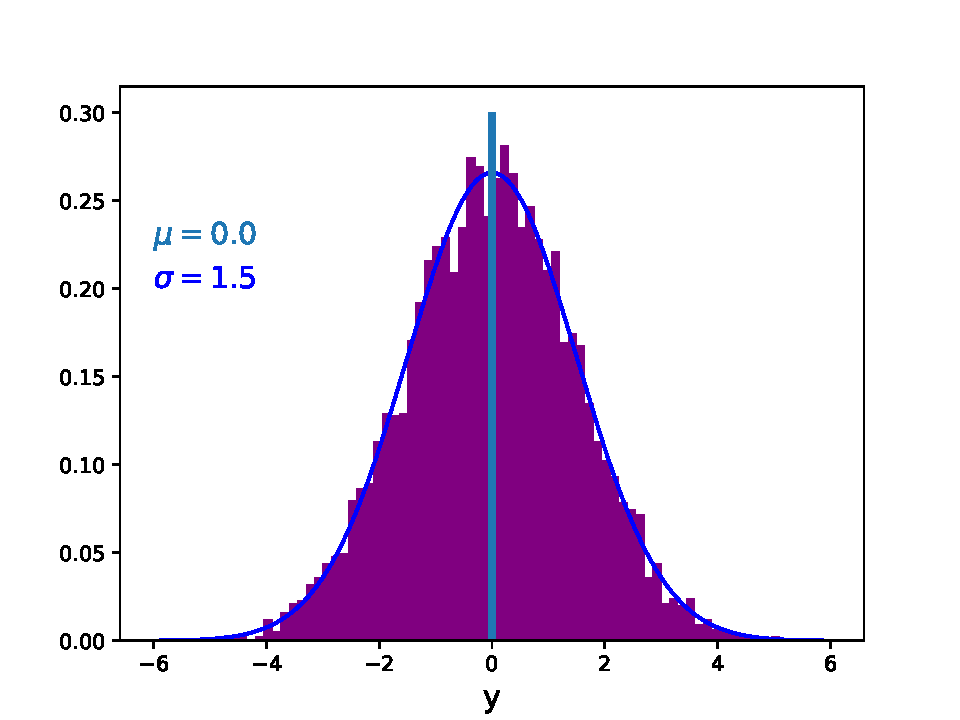
\includegraphics[scale=0.4]{gaussian_1d.pdf}
  \end{figure}

\end{frame}

\begin{frame}
  \frametitle{\secname}

  Loi Gaussienne multidimensionnelle (vecteur Gaussien): Distribution \coloredemph{jointe} d'un vecteur $d$-dimensionnel dont les \coloredemph{marginales} sont Gaussiennes (unidimensionnelles).
  \begin{equation*}
    \vectorx{Y} := [ y_1, \dots, y_d ]^\top  \sim \mathcal{N}(\vectorx{\mu} , \matrixx{\Sigma}) =  \frac{1}{\sqrt{(2 \pi)^d \det |\matrixx{\Sigma}|}} e^{-\frac{1}{2}(\vectorx{y - \mu})^\top \matrixx{\Sigma}^{-1} (\vectorx{y - \mu})}
  \end{equation*}
% 
  \begin{enumerate}
    \item $\vectorx{\mu} \in \mathbb{R}^d$: \coloredemph{vecteur moyen} $\implies \mu_j$: moyenne de la Gaussienne $y_j$
    \item $\matrixx{\Sigma} \in \mathbb{R}^{d \times d}$ définie positive\footnote{i.e. $\vectorx{a}^\top \matrixx{\Sigma} \vectorx{a} > 0$ (donc symmétrique)}: \coloredemph{matrice de covariance}
  \end{enumerate}
% 
  \pause
  \begin{equation*}
    \matrixx{\Sigma}
    =
    \begin{pmatrix} 
      \Sigma^2_{1}  & \Sigma_{{1}{2}} &  \cdots & \Sigma_{{1}{d}} \\
      \Sigma_{{2}{1}} & \ddots          & \cdots  & \vdots \\
      \vdots          & \vdots          & \ddots  & \vdots \\
      \Sigma_{{d}{1}} & \cdots          & \cdots  &  \Sigma^2_{d} 
      \end{pmatrix}
    \implies
    \left\{
      \begin{array}{ll}
        \Sigma_j  : \text{écart-type} \text{ de } y_j\\
        \Sigma_{ij} : \text{covariance entre } y_i \text{ et } y_j
      \end{array}
    \right.
  \end{equation*}

  % $\mathcal{N}(\mu_1, \Sigma_1^2) \dots \mathcal{N}(\mu_d, \Sigma_d^2)$.
\end{frame}

% d=2, low correlation
\begin{frame}
  Cas $d=2$:
  \begin{equation*}
    \vectorx{\mu}
    =
    \begin{pmatrix}
      \mu_1 \\
      \mu_2
    \end{pmatrix},
    \quad
    \matrixx{\Sigma}
    =
      \begin{bmatrix}
        \Sigma_{1} & \Sigma_{12} \\
        \Sigma_{21} & \Sigma_{2}
      \end{bmatrix}
    =
      \begin{bmatrix}
        1.5 & \color{red}\rho = -0.3 \\
        \color{red}\rho = -0.3 & 1.5
      \end{bmatrix}
  \end{equation*}
% 
  \begin{figure}
    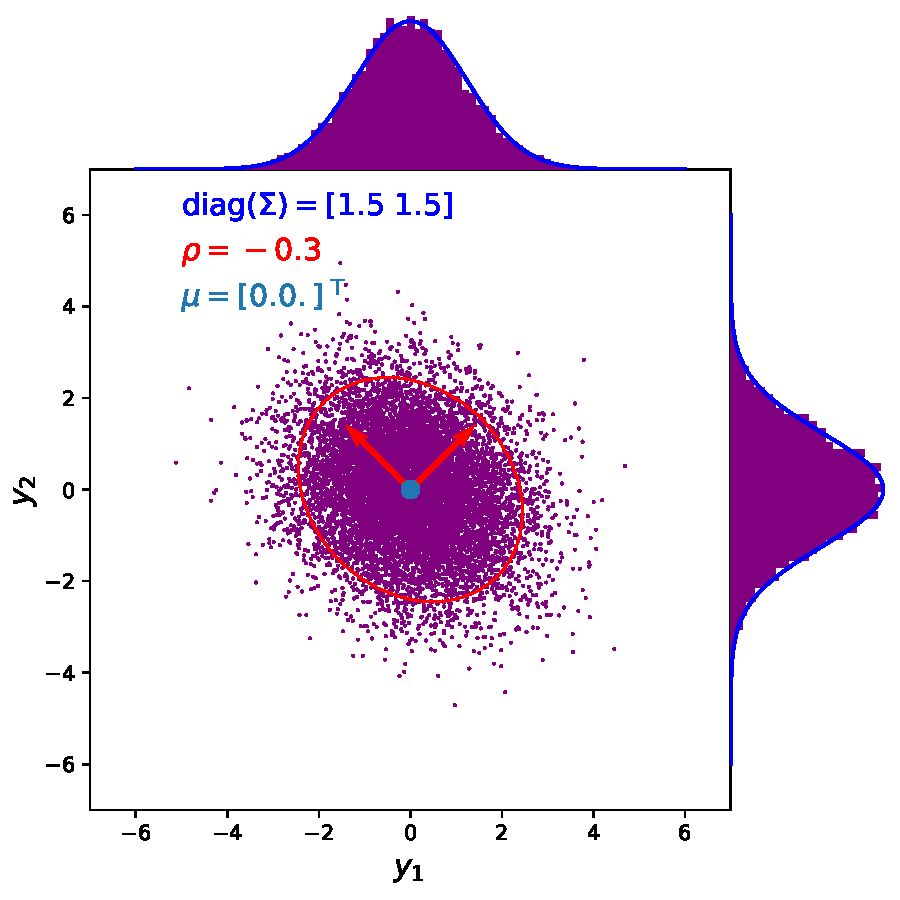
\includegraphics[scale=0.4]{gaussian_2d_rho_low.pdf}
  \end{figure}
\end{frame}

% d=2, high correlation
\begin{frame}
  Cas $d=2$:
  %
  \begin{equation*}
    \vectorx{\mu}
    =
    \begin{pmatrix}
      \mu_1 \\
      \mu_2
    \end{pmatrix},
    \quad
    \matrixx{\Sigma}
    =
      \begin{bmatrix}
        \Sigma_{1} & \Sigma_{12} \\
        \Sigma_{21} & \Sigma_{2}
      \end{bmatrix}
    =
      \begin{bmatrix}
        1.5 & \color{red}\rho = 1.1 \\
        \color{red}\rho = 1.1 & 1.5
      \end{bmatrix}
  \end{equation*}
% 
  \begin{figure}
    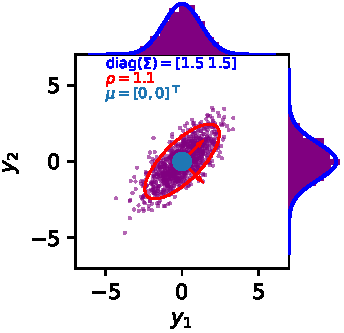
\includegraphics[scale=0.4]{gaussian_2d_rho_high.pdf}
  \end{figure}
\end{frame}

% d=2, zero correlation
\begin{frame}
  Cas $d=2$:
  %
  \begin{equation*}
    \vectorx{\mu}
    =
    \begin{pmatrix}
      \mu_1 \\
      \mu_2
    \end{pmatrix},
    \quad
    \matrixx{\Sigma}
    =
      \begin{bmatrix}
        \Sigma_{1} & \Sigma_{12} \\
        \Sigma_{21} & \Sigma_{2}
      \end{bmatrix}
    =
      \begin{bmatrix}
        1.5 & \color{red}\rho = 0 \\
        \color{red}\rho = 0 & 1.5
      \end{bmatrix}
  \end{equation*}
% 
  \begin{figure}
    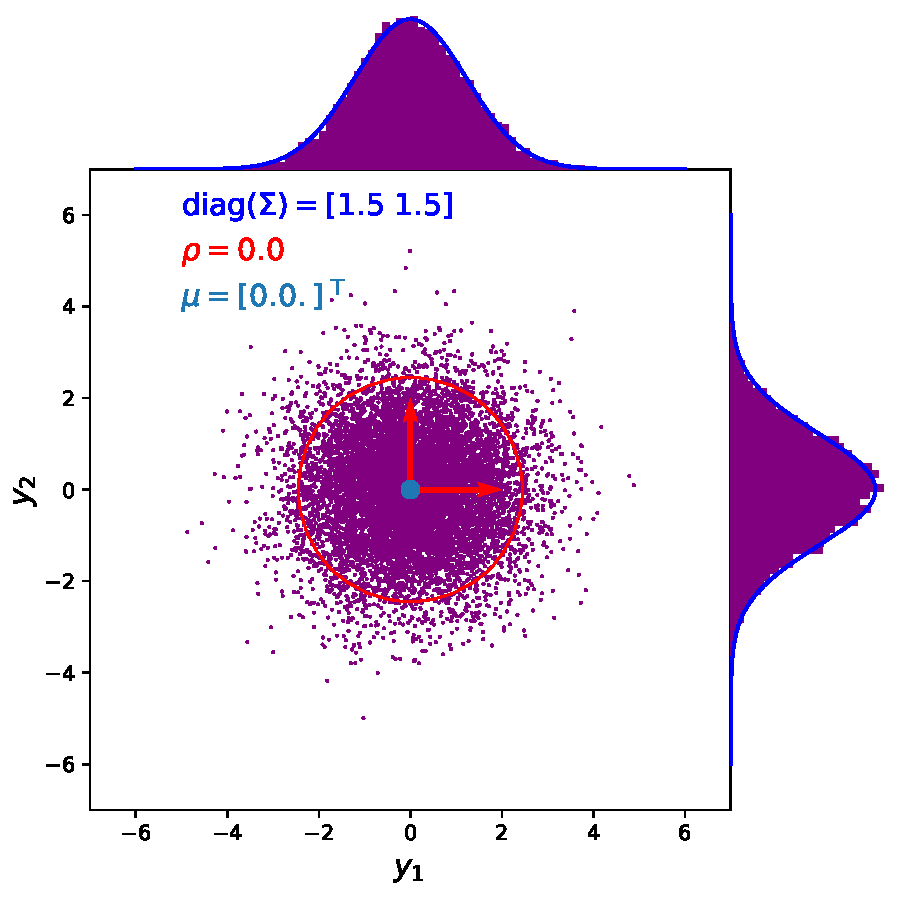
\includegraphics[scale=0.4]{gaussian_2d_rho_null.pdf}
  \end{figure}
\end{frame}

% d=5, high correlation: scatter and index plots
\begin{frame}
  Cas $d=2$:
  %
  \begin{equation*}
    \vectorx{\mu}
    =
    \begin{pmatrix}
      0 \\
      0 \\
      \dots
    \end{pmatrix},
    \quad
    \matrixx{\Sigma}
    =
    \begin{bmatrix}
      1.5 & 0.99 & \color{lightgray}0.98 & \color{lightgray}0.96 & \color{lightgray}0.94 \\
      0.99 & 1.5 & \color{lightgray}0.99 & \color{lightgray}0.98 & \color{lightgray}0.96 \\
      \color{lightgray}0.98 & \color{lightgray}0.99 & \color{lightgray}1.5 & \color{lightgray}0.99 & \color{lightgray}0.98 \\
      \color{lightgray}0.96 & \color{lightgray}0.98 & \color{lightgray}0.99 & \color{lightgray}1.5 & \color{lightgray}0.99 \\
      \color{lightgray}0.94 & \color{lightgray}0.96 & \color{lightgray}0.98 & \color{lightgray}0.99 & \color{lightgray}1.5
      \end{bmatrix}
  \end{equation*}
  %
  \begin{figure}[ht]
    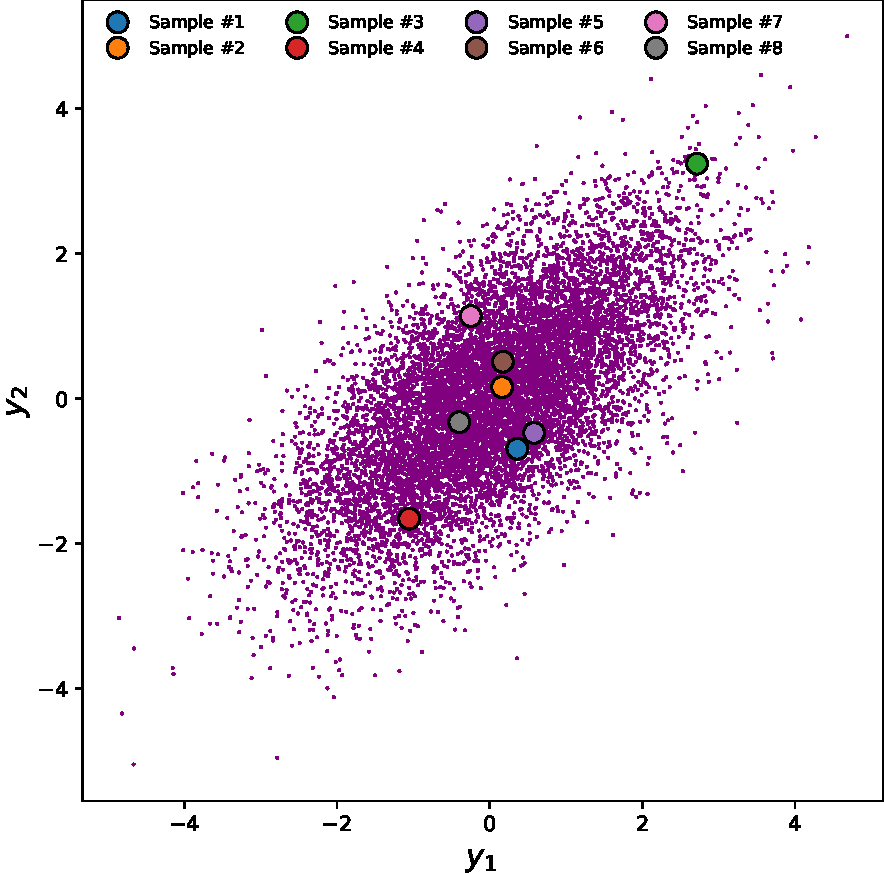
\includegraphics[scale=0.3]{gaussian_2d_2outof5.pdf}
    $\Longleftrightarrow$
    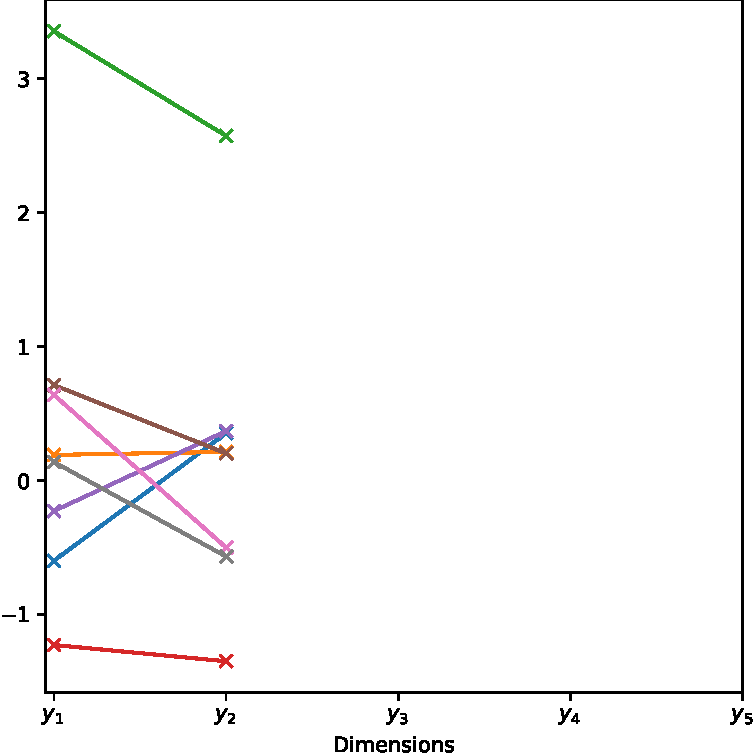
\includegraphics[scale=0.3]{gaussian_2d_valuevsindex.pdf}
    \caption{Dimensions $j=1, 2$. Gauche: \textcolor{violet}{$10^4$} $+8$ échantillons. 
    Droite: $8$ \coloredemph{mêmes} échantillons.}
  \end{figure}
\end{frame}

% d=5, high correlation: scatter and index plots
\begin{frame}
  Cas $d=5$:
  %
  \begin{equation*}
    \vectorx{\mu}
    =
    \begin{pmatrix}
      0 \\
      0 \\
      \dots
    \end{pmatrix},
    \quad
    \matrixx{\Sigma}
    =
    \begin{bmatrix}
      1.5 & 0.99 & 0.98 & 0.96 & 0.94 \\
      0.99 & 1.5 & 0.99 & 0.98 & 0.96 \\
      0.98 & 0.99 & 1.5 & 0.99 & 0.98 \\
      0.96 & 0.98 & 0.99 & 1.5 & 0.99 \\
      0.94 & 0.96 & 0.98 & 0.99 & 1.5
      \end{bmatrix}
  \end{equation*}
  %
  Chaque courbe est un tirage de $\mathcal{N}(\vectorx{\mu} , \matrixx{\Sigma})$
  \begin{figure}[ht]
    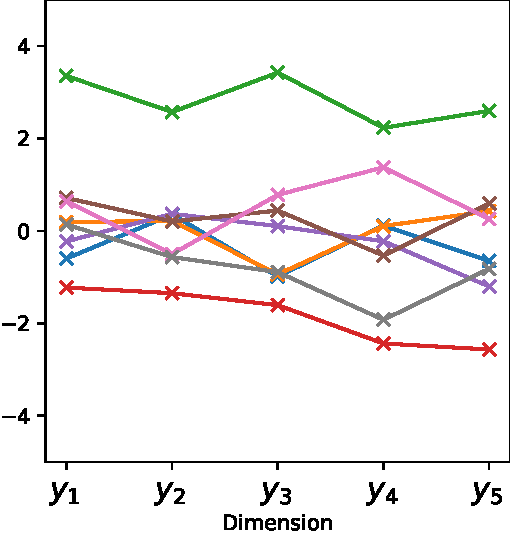
\includegraphics[scale=0.3]{gaussian_5d_valuevsindex.pdf}
    \caption{$8$ échantillons, dimensions $j=1, \dots, 5$}
  \end{figure}
\end{frame}

% d=50, high correlation: scatter and index plots
\begin{frame}
  Cas $d=50$:
  %
  \begin{equation*}
    \vectorx{\mu}
    =
    \begin{pmatrix}
      0 \\
      0 \\
      \dots
    \end{pmatrix},
    \quad
    \matrixx{\Sigma}
    =
    \scalemath{0.65}{
      \begin{bmatrix}
        1.5 & 0.998 & 0.993 & 0.986 & 0.975 & 0.962 & 0.946 & 0.927 & \cdots \\
        0.998 & 1.5 & 0.998 & 0.993 & 0.986 & 0.975 & 0.962 & 0.946 & \cdots \\
        0.993 & 0.998 & 1.5 & 0.998 & 0.993 & 0.986 & 0.975 & 0.962 & \cdots \\
        0.986 & 0.993 & 0.998 & 1.5 & 0.998 & 0.993 & 0.986 & 0.975 & \cdots \\
        0.975 & 0.986 & 0.993 & 0.998 & 1.5 & 0.998 & 0.993 & 0.986 & \cdots \\
        0.962 & 0.975 & 0.986 & 0.993 & 0.998 & 1.5 & 0.998 & 0.993 & \cdots \\
        0.946 & 0.962 & 0.975 & 0.986 & 0.993 & 0.998 & 1.5 & 0.998 & \cdots \\
        0.927 & 0.946 & 0.962 & 0.975 & 0.986 & 0.993 & 0.998 & 1.5   \\
        \hdots & \hdots & \hdots & \hdots & \hdots & \hdots & \hdots & \hdots & 1.5
      \end{bmatrix}
    }
  \end{equation*}
  Chaque courbe est un tirage de $\mathcal{N}(\vectorx{\mu} , \matrixx{\Sigma})$
  %
  \begin{figure}[ht]
    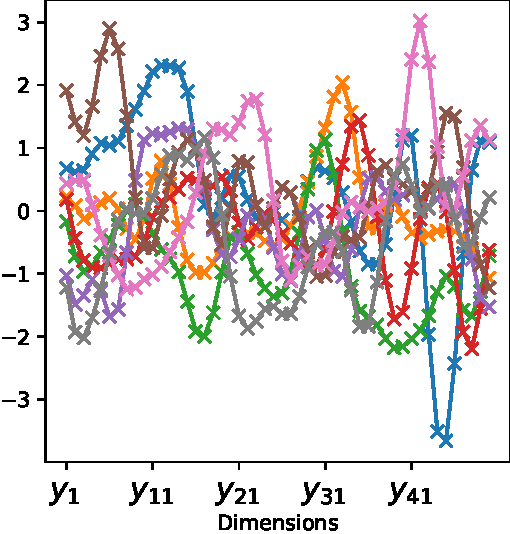
\includegraphics[scale=0.3]{gaussian_50d_valuevsindex.pdf}
    \caption{$8$ échantillons, dimensions $j=1, \dots, 50$}
  \end{figure}
\end{frame}
%

\begin{frame}
  Cas $d=\infty$: chaque courbe est une \coloredemph{collection infinie} d'échantillons Gaussiens.
  \begin{enumerate}
    \item $\vectorx{\mu}$: vecteur de taille infinie
    \item $\matrixx{\Sigma}$: une fonction de covariance
  \end{enumerate}
  %
  % Définition d'un processus Gaussien
\end{frame}
%========== Motivations ==================%
% \section{Motivations}
% Où est-ce rencontre-t-on des processus stochastiques ?
% Gaussiens ?

\section[short]{}
\end{document}